\RequirePackage[T1]{fontenc}
\documentclass[conference]{IEEEtran}
\usepackage{amsmath,amssymb}
\usepackage{newtxtext,newtxmath}
\usepackage{graphicx}
\graphicspath{{paper/figures/}{figures/}}
\usepackage{booktabs}
\usepackage{balance}
\usepackage{url}
\usepackage[hidelinks]{hyperref}
\title{Consequa-X: An Evidence and Intervention Protocol for Consequential Agent Actions}
\author{\IEEEauthorblockN{Devrajsinh Jhala}\IEEEauthorblockA{Independent Researcher}}
\begin{document}
\raggedbottom
\maketitle

\begin{abstract}
A lost acknowledgement can turn a successful agent action into a duplicate
when retried. Consequa-X separates reported assessment, verified state and
source-supported effect origin, preserving observation-specific provenance
and explicit unknown verdicts. Its research adapter declares an on-reach
intervention game and refusal-aware accounting around existing contrastive
and permutation Shapley estimators. Across 2,048 scripted-simulator sampling
trials, all 655,360 planned branches were retained. At one retry coefficient,
normal intervals covered the reference in 118/128 trials; Hoeffding bounds
covered in 128/128 but detected its sign in 8/128. A three-model factual study
completed 503/504 episodes using 896 local calls. An equally informed,
independently implemented reference agreed throughout; state verification
made 431 correct definite claims, compared with 53 errors among 201
response-only claims. A same-evidence local judge made 9 errors among 60
definite state claims across 84 traces. Model-free transfer retained 656
retail/airline task-control cells and 900 operation captures, separating
native whole-task DB equality from immediate field contracts. A pinned native
Causal Agent Replay comparison retained 1,024 paired groups: all 640 eligible
point vectors agreed exactly; 384 pairs remained unavailable. A collector
deviation limits refused-attempt accounting in 64 already ineligible groups.
These experiments use Consequa-X 1.1.0. Separately frozen offline migration
to 2.0 preserved canonical conclusions on all 503 retained traces, including
72 unknown states, while diagnosis codes changed on 275. These conditional
results support an inspectable protocol, without estimator novelty or general
superiority; real-service effectiveness and independent human validation
remain open.
\end{abstract}

\begin{IEEEkeywords}
agent systems, outcome verification, evidence provenance, counterfactual replay,
software artifacts, uncertainty
\end{IEEEkeywords}

\section{Introduction}
A consequential tool operation has distinct stages: selection, dispatch,
execution, response, reported assessment and external observation. A service
can commit an effect before its acknowledgement is lost. Retrying can create
another effect unless the logical operation's identity and idempotency semantics
are retained. Conversely, a successful response can coexist with an incomplete
or incorrect effect. Explaining such runs requires more than reading the last
tool response or the agent's prose.

State satisfaction and effect origin also differ. An external refund may
satisfy the requested balance or count while remaining unlinked to this agent.
A source-supported origin link is a provenance claim; it does not establish
counterfactual necessity. A replay effect is a separate claim about a declared
intervention, continuation policy and outcome distribution.

Consequa-X makes these distinctions inspectable. Its core contains typed
records, schema validation, application verification and evidence-only
explanation. Its research adapters provide isolated refund worlds, public-only
policy inputs, a local Ollama adapter and bounded replay experiments. Reported
assessments are captured outputs, not measurements of hidden reasoning.

The paper centers three testable protocol claims:
\begin{enumerate}
\item \textbf{C1: State and origin remain separate.} A satisfied contract can
retain an other-actor or unknown origin. Successive readbacks retain their own
supporting witnesses rather than transferring provenance between observations.
Verification and graph tests exercise external-actor, missing-provenance and
conflicting-witness cases; the local validation contains an other-actor example.
\item \textbf{C2: The replay game is explicit.} On-reach semantics define how
normal early termination treats later requested holds. Strict and on-reach
results remain separate. Analytic enumeration and the variable-length controls
test this distinction; Appendix~\ref{app:games} states its formal scope.
\item \textbf{C3: Refusal remains observable.} Every planned branch is retained
with call accounting; incomplete evidence or an invalid draw refuses affected
estimates. The repeated-sampling study accounts for all 655,360 slots and
reports availability beside numerical accuracy.
\end{enumerate}
These are implementation and declared-game claims. The contribution combines
them in a portable protocol around existing estimators. The matched factual
study below finds exact agreement with an equally informed independent
reference, supporting implementation correctness without empirical advantage.
Figure~\ref{fig:architecture} separates the captured-evidence core from the
explicitly invoked research replay path.

\begin{figure*}[t]
\centering
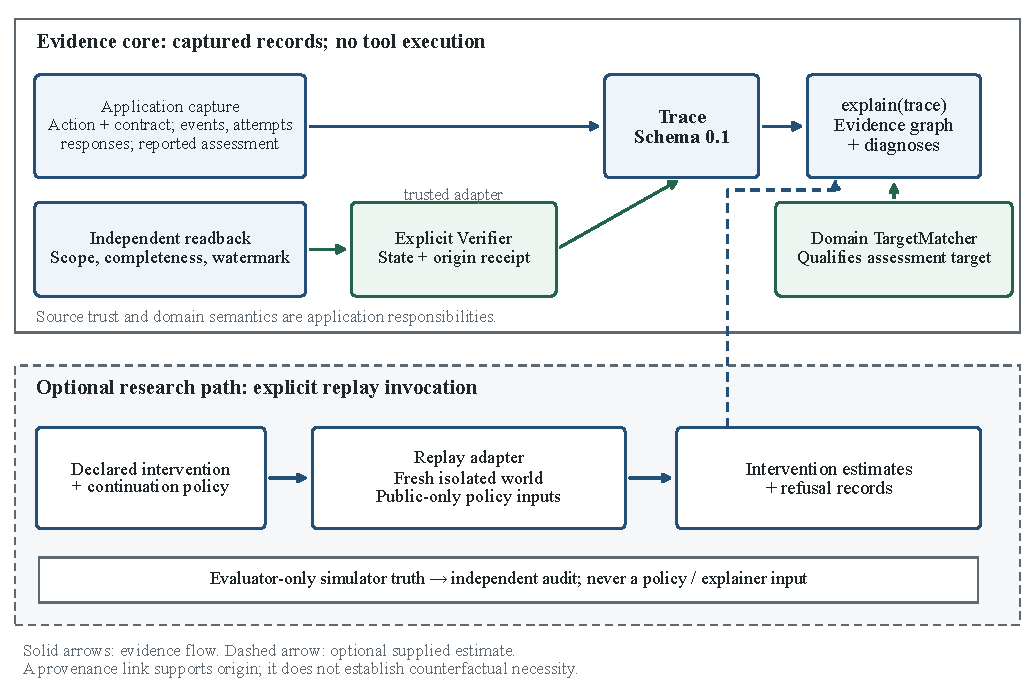
\includegraphics[width=\textwidth]{diagram-evidence-architecture.pdf}
\caption{Evaluated 1.x evidence flow and trust boundaries. Application verifiers interpret
independent readback; explanations use captured evidence. Explicitly invoked
replay can supply estimates, while evaluator truth remains audit-only. Source
trust and domain semantics remain application responsibilities.}
\label{fig:architecture}
\end{figure*}

\section{Related Work}
Causal Agent Replay (CAR) performs same-policy interventions on recorded
decisions, evaluates user-specified outcomes and uses contrastive suffix and
permutation Shapley attribution~\cite{car}. Consequa-X implements an independent
binary adaptation with its own typed-world, evidence and refusal boundaries.
Applying a verified outcome to replay is therefore not an estimator novelty
claim. Policy-Conditioned Counterfactual Credit studies changes in final
verified success under specified interventions and a continuation
policy~\cite{pccc}; its learning objective differs from post-hoc external-effect
diagnosis, but verified targets and valid interventions are shared concerns.

CausalLoss-Fin jointly intervenes on agent decisions and repairable
infrastructure messages~\cite{causalloss}. Its deterministic programmatic
evaluation limits transfer to stochastic language policies, but it already
occupies the broad combination of financial effects and joint decision/fault
attribution. A future comparison must expose applicable variables to every
method rather than charge omitted infrastructure effects to decisions.

Verified Tool Calls distinguishes acknowledgements from independently checked
effects and uses unknown postcondition conclusions~\cite{verified}.
Callability Is Not Operability studies controlled interface ambiguity and
terminal agent claims~\cite{operability}. Three-valued verification and
response/effect separation are foundations and comparison requirements here.
These targeted primary-source checks do not constitute a systematic review or
an independent reproduction of those papers' empirical results.

Who\&When attributes failed multi-agent runs to an agent and decisive step
from annotated logs~\cite{whoandwhen}; this differs from verifying a particular
external effect from an independent witness. PROV-DM already represents entities,
activities, agents and responsibility~\cite{prov}. Consequa-X is neither a new
general provenance model nor a PROV conformance implementation. Its narrower
contribution is an executable protocol linking temporal contracts, observation
witnesses, separate origin verdicts and explicit refusal.

Agent--tool anomaly work already separates external events from runtime
observations, including exogenous effects~\cite{agenttool}; LIMBO grades
committed-effect histories and analyzes late commits~\cite{limbo}. Response/effect
separation and effect ledgers are therefore prior concepts. Our study audits
a particular protocol rather than establishing a safer recovery controller.
LIMBO's late-commit argument assumes a keyless, non-idempotent write with no
known finite in-flight bound and finite task-completion time. Under those
conditions, bounded watermark polling cannot guarantee exactly-once execution.
Idempotence and eventual consistency are established systems concerns~\cite{helland,vogels}.

AppWorld, ToolSandbox and $\tau$-bench already evaluate world-state outcomes
or stateful trajectories~\cite{appworld,toolsandbox,taubench}. The maintained
tau3 task corpus supplies the retail/airline tool-state transfer experiment
below~\cite{tau3tasks}; AppWorld, ToolSandbox and autonomous benchmark
evaluation remain future comparisons. For statistics, known binomial Wald-interval limitations~\cite{brown} motivate
careful interval checks but do not by themselves establish paired-Shapley
undercoverage. Modern bounded-mean betting intervals~\cite{betting} are planned
comparators, with the sampling unit and stopping rule still requiring explicit
validation for this replay setting.

\section{Evidence Protocol and Core Interfaces}
\subsection{Objects, contracts and trust}
The empirical studies below evaluate the versioned 1.x reference
implementation and schema 0.1, with study-specific source pins. The current
2.x line uses schema 1.0, multiple actions per trace and explicit time
bases. It refuses direct loading of 0.1 traces and provides an explicit,
conservative migration path. Historical interfaces and results must therefore
remain distinct from current product capabilities~\cite{experimentartifact,artifact}.

Let $H$ be visible history, $A$ a logical action, $E$ an execution attempt,
$R$ its response, $B$ a timestamped reported assessment and $O$ an independent
readback observation. A contract $C$ declares payload, count, deadline and
stability horizon. The verifier conclusion $V(C,O)$ is satisfied, violated or
unknown. Origin is separately confirmed, other actor or unknown. Evaluator-only
simulator truth never becomes a policy or explainer input.

The built-in refund predicate uses integer currency minor units. An eligible
effect matches payment, amount and currency, commits in the declared time
window and persists through the horizon. Exact-count contracts also constrain
the count during the stability interval. A stale watermark or inadequate scope
and completeness yields unknown rather than a confident absence claim.
Source authority, scope, completeness and watermark declarations remain trusted
adapter inputs. Schemas and hashes validate structure and changed bytes, not
source authenticity or real transactional guarantees.
Figure~\ref{fig:timeout} illustrates why a response and a reported assessment
cannot substitute for a horizon-covering outcome observation.

\begin{figure*}[t]
\centering
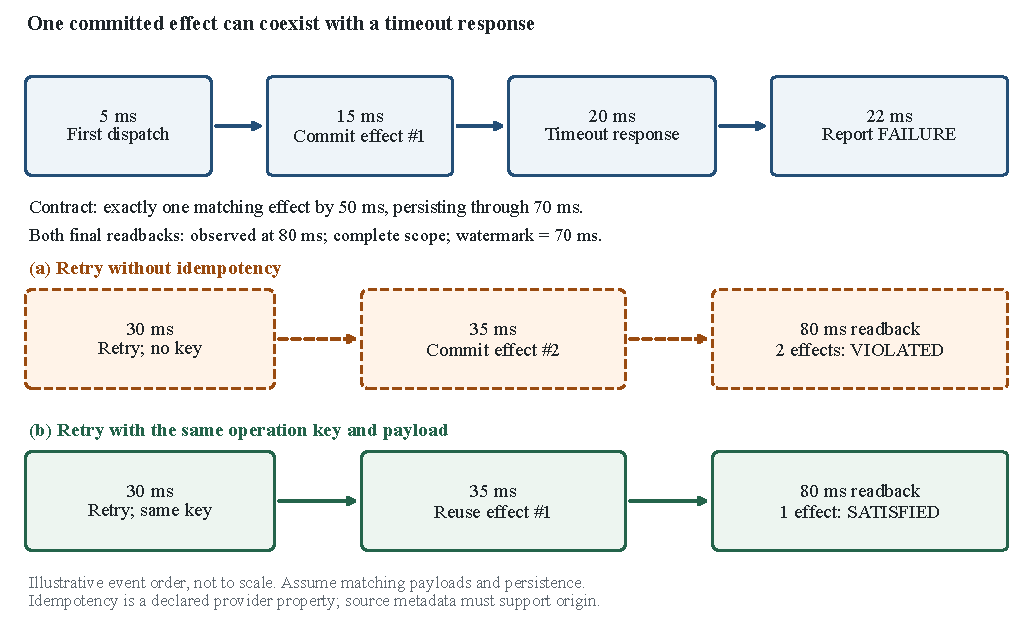
\includegraphics[width=\textwidth]{diagram-timeout-retry.pdf}
\caption{Illustrative timeout-after-commit sequence. A committed effect precedes
a timeout and reported failure. An unsafe retry creates a duplicate; reusing the
same provider-scoped idempotency key and payload preserves one effect. Complete
final readback covers the stability horizon. Arrows show event order, and times
are illustrative rather than sampled observations.}
\label{fig:timeout}
\end{figure*}

\subsection{Reusable application boundary}
The evidence core can operate on a production application's captured records
without any replay. A read-only adapter obtains independent observations;
verification returns state and origin conclusions, and explanation renders the
supporting evidence. This path requires neither simulator reset nor a second
execution of a consequential action.

Applications can supply an explicit read-only verifier through
\texttt{verify(action, observation, verifier=...)}. The wrapper checks receipt
type, contract identity, observation identity, source, watermark and timing.
Domain predicate semantics, authentication and read-only adapter behavior are
the application's responsibility. There is no evaluation of arbitrary predicate
strings. An offline artifact-delivery example constructs captured records and
checks independently read-back content digests without importing the refund
simulator or executing writes.

In the evaluated 1.x interface, \texttt{explain(trace)} reads a captured
verification and performs no replay.
Refund target matching is built in; other predicates receive a neutral
explanation unless a trusted domain matcher explicitly qualifies attributable
effects against payload and temporal rules. Matchers can return only unique
IDs within the receipt's attributable IDs. Unknown receipts are not interpreted
as target matches. A qualified provenance link still is not a causal effect.
In 2.0, verifiers record target-effect IDs and findings in each receipt;
explanation consumes those records per action rather than invoking a separate
target matcher. This API change requires explicit migration and version-specific
conformance checking.

\subsection{Successive witnesses and graph meanings}
Repeated readbacks can disagree about the same effect identifier. The graph
therefore retains observation-specific witnesses and an identity-only shared
effect node. Dispatch-to-effect edges attach to the witness supplying origin
metadata; verification edges use witnesses in that receipt's own observations.
A later conflicting actor, corrected payload or reversal cannot overwrite an
earlier witness and inherit its unqualified origin link. Shared identifiers do
not authenticate or reconcile the records. Estimated-influence edges require
captured event identifiers and an explicitly supplied intervention estimate.

\section{Replay Targets, Games and Uncertainty}
\subsection{Targets and conditional suffix effects}
The refund adapter exposes three targets: initial action selection, global
state-contract satisfaction and action-linked consequence. A known global
violation is false for the linked target. Satisfied state with exclusively
external qualifying effects is false for that target; insufficient provenance
can instead yield unknown. The linked target combines global satisfaction and
qualifying operation-linked witnesses rather than reconstructing an agent-only
world. Unknown observations do not acquire numeric labels.

For known binary target $Z$, set bad outcome $X=1-Z$. Prefix replay holds
factual decisions before position $k$ and resamples the suffix. With one
observed factual bad label $x_f$, the conditional estimand is
\begin{equation}
\gamma_k = \mathbb{E}[X\mid \text{prefix held, suffix resampled at }k]-x_f.
\end{equation}
The factual term is one observed constant, not a population rate estimate.
This factual-anchored target answers: how often would a fresh suffix avoid the
bad outcome observed in this episode? It is useful for episode diagnosis, but
does not estimate the effect of changing one decision against an independently
resampled original arm. That population contrast would instead compare two
expectations, for example $\mathbb{E}[X\mid\text{hold }k]-
\mathbb{E}[X\mid\text{resample }k]$, with the other conditions declared.
Neither estimand is generally preferable; they answer different questions and
have different sampling costs. Here negative $\gamma_k$ indicates rescue
relative to the observed episode. An earlier irrelevant position can have a
nonzero suffix effect because its suffix contains a later stochastic choice.
The \emph{pivot} is the latest position with negative population suffix effect
under this definition. The retained nominal selector attempts to detect that
position only if all planned positions are estimable. Its pointwise intervals
give no simultaneous or post-selection coverage guarantee; selected pivots are
exploratory diagnostics rather than unique causes.

\subsection{Held-decision coalition games}
Let $N$ be reached factual positions. Coalition $S$ requests holding captured
decisions at positions in $S$; other decisions are sampled. Reached held
decisions must match the typed public stage. In the \emph{strict} game, an
earlier termination leaving a requested held position unreachable invalidates
the draw. Finite samples avoiding invalidity do not define the population game.

The separate \emph{on-reach} game treats requested positions beyond a normal
termination as inactive and uses the actual completed episode. Reached
incompatible operations remain invalid; provider failures and exhausted budgets
are not normal inactivity. This is an explicit alternative game, not a repair
of retained strict results.

For a defined game $v(S)=\mathbb{E}[X\mid S]$, signed Shapley values allocate
the held-decision effect~\cite{shapley}:
\begin{equation}
\phi_i = \sum_{S\subseteq N\setminus\{i\}}
\frac{|S|!(|N|-|S|-1)!}{|N|!}\,[v(S\cup\{i\})-v(S)].
\end{equation}
Fresh forward/reverse permutation walks form one paired contribution vector.
Independent empty/full draws diagnose the endpoint scale. Values are signed
allocations under the declared game, not normalized responsibility shares.
Positive values mean holding the factual decision increases bad outcomes;
negative values mean it is protective.

\subsection{Intervals and refusals}
Contrastive defaults use exact binomial Clopper--Pearson bounds translated by
$-x_f$~\cite{clopperpearson}. Signed pair observations lie in $[-1,1]$; the default
Hoeffding half-width for $P$ independent pairs and failure allowance $\alpha$
is~\cite{hoeffding}
\begin{equation}
h=\sqrt{\frac{2\log(2/\alpha)}{P}}.
\end{equation}
This is the half-width before clipping the interval to $[-1,1]$.
Endpoint differences use two exact binomial marginals with a split failure
allowance. Each marginal has confidence $1-\alpha/2$; the difference interval
is $[L_f-U_e,U_f-L_e]$. The union bound requires valid marginal bounds, not
independence between the two arms. Bootstrap and normal intervals remain
explicit legacy comparators.
These are standard conditional methods with sampling assumptions and precision
costs, not distribution-free guarantees for dependent model continuations.
All reported coefficient intervals are pointwise. For a predeclared family
of $m$ valid marginal intervals, allocating failure probability $\alpha/m$ to
each would give a Bonferroni family guarantee without independence across
positions. That adjustment was not used in these retained studies. A nominal
latest-rescue selection therefore does not inherit a 95\% family guarantee.
Variance-adaptive or betting-based bounded-mean methods~\cite{betting} are
relevant future comparators; the present results do not establish that
Hoeffding is optimal or that conservative uncertainty must have this width.

Replay requires a resettable, isolated simulator or a validated digital twin.
It must not reissue real refunds or other consequential production writes.
The studies below reset a scripted payment simulator, whose fidelity is a
separate assumption; the evidence-only production path does not require it.
Held replies consume no fresh calls;
every attempted fresh call, including a provider/protocol failure, consumes
budget. Every planned branch remains recorded. Unknown, invalid, failed and
unstarted branches are not dropped or redrawn; affected estimates are refused.
Targets and interval variants reuse captured evidence without extra policy calls.

\subsection{Analytic refund reference}
Consider the declared on-reach refund mechanism with adequate budget, complete
horizon-covering readback and, for the linked target, sufficient provenance.
The planted factual decisions are selection $s$, retry $r$ and final stop $t$.
Fresh selection occurs with probability $p$ and fresh timeout retry with
probability $q$ under the declared independent choice law. The first attempt
commits despite its timeout; without idempotency, a retry commits a second
refund. Exactly one effect therefore occurs with probability $p(1-q)$.
For the consequence bad-outcome game, the four relevant coalition values are
\begin{equation}
\begin{aligned}
v(\varnothing)&=1-p(1-q), & v(\{s\})&=q,\\
v(\{r\})&=1, & v(\{s,r\})&=1.
\end{aligned}
\end{equation}
The final stop is a dummy: adding $t$ changes none of these values. Averaging
the two orders of the active players gives
\begin{equation}
\begin{aligned}
\phi_s&=-\tfrac12(1-p)(1-q),\\
\phi_r&=\tfrac12(1+p)(1-q),\qquad \phi_t=0.
\end{aligned}
\end{equation}
Their sum is the endpoint difference $p(1-q)$; the selection/retry interaction
$v(\{s,r\})-v(\{s\})-v(\{r\})+v(\varnothing)$ is $(1-p)(1-q)$.
At $p=q=0.5$, these are shares $[-0.125,0.375,0]$, endpoint 0.25 and
interaction 0.25. With idempotency, any selected refund creates one effect,
so consequence shares become $[-(1-p),0,0]$, as for initial action selection;
the interaction is zero. These are population references derived from the
declared mechanism, not fitted to sampled outcomes. A call cap can refuse the
finite estimate despite a defined ideal reference. Unknown evidence or strict
unreachable-held decisions do not acquire numeric references from these forms.

A standalone standard-library check uses exact rational arithmetic on a
five-by-five $(p,q)$ grid, two idempotency settings and two targets: 100 control
cases. It checks all coalition values and six permutation orders against these
forms without importing the framework or reading sampled study data. This
checks the stated mathematical law, not simulator execution or sampling validity.

\section{Audited Evaluation}
\subsection{Original calibration and finite analysis}
The \emph{protective-stop} fixture forces the factual timeout decision to stop
after one committed refund. Fresh continuations retry with probability $q$,
so resampling can introduce a duplicate. The \emph{retry-pivot} fixture instead
forces a factual retry; its timeout position is the latest population rescue
position when $0<q<1$. These are planted scripted decisions, not model-derived
causal labels.

The original development study retained 1,280 trials across ten specified
mechanisms, with 128 repetitions. Of 223,232 planned branches, 198,690
completed, 4,062 were invalid, 256 failed at the deliberate cap and 20,224
were unstarted. Standalone audit scripts checked raw evidence, seeded outcomes,
statistics and accounting. Table~\ref{tab:original} reports a preselected
protective-stop consequence position with 128 available, reference-eligible
estimates in each row.

\begin{table}[t]
\caption{Original protective-stop consequence position: nominal 95\%
percentile-bootstrap contrastive and normal paired-Shapley coverage.
Each entry has 128 available, reference-eligible trials.}
\label{tab:original}
\centering
\begin{tabular}{lrr}
\toprule
Retry $q$ & Contrastive covered & Shapley covered\\
\midrule
0.1 & 100/128 & 107/128\\
0.5 & 122/128 & 121/128\\
0.9 & 103/128 & 103/128\\
\bottomrule
\end{tabular}
\end{table}

Separate finite-distribution calculations yielded protective-stop normal pair
coverage of 83.7775\% at $q=0.1,0.9$ and 92.6377\% at $q=0.5$ for 16 pairs.
For interior Bernoulli $q$, homogeneous draws force an empirical percentile
bootstrap interval to a point, giving coverage ceiling
$1-q^K-(1-q)^K$. At $K=16$ and $q=0.1,0.9$, this is about 81.47\%.
These findings concern the specified adaptation; they do not establish
coverage of upstream CAR implementations.

\subsection{Shared-draw conservative comparison}
A separately frozen follow-up retained 384 trials across twelve cases,
66,048 planned branches and 87,054 actual scripted calls. Variants reused
the same points, draws, seeds and refusals. Exact probability weights over
sample counts 8,16,32,64 and eleven probabilities yielded minimum grid
coverage 7.72\% for the limiting empirical percentile bootstrap, 85.15\% for
Wilson and 96.68\% for Clopper--Pearson. The bootstrap grid is its
infinite-resample limit, distinct from the replay's finite seeded bootstrap.

\begin{table}[t]
\caption{Fresh protective-stop shared-draw coverage: 32 trials per row.
Bootstrap/exact-binomial intervals cover the contrastive effect;
normal/Hoeffding intervals cover the paired-Shapley coefficient.}
\label{tab:followup}
\centering\footnotesize
\begin{tabular}{lrrrr}
\toprule
$q$ & Bootstrap & Exact binomial & Normal & Hoeffding\\
\midrule
0.1 & 26/32 & 31/32 & 23/32 & 32/32\\
0.5 & 31/32 & 32/32 & 32/32 & 32/32\\
0.9 & 31/32 & 32/32 & 29/32 & 32/32\\
\bottomrule
\end{tabular}
\end{table}

Table~\ref{tab:followup} is the protective-stop timeout position, not every
case. The full summary includes exact-binomial coverage 30/32 for a retry-pivot
case. Finite observed coverage can fall below nominal despite a conservative
population method. At $q=0.1$, mean normal versus Hoeffding width was about
0.180 versus 1.358; at $q=0.5$, 0.344 versus 1.184. Hoeffding detected the
negative reference sign in 0/32 trials at both weaker settings, and 32/32 at
$q=0.9$. Wider intervals therefore impose a substantial detection cost.

The standalone saved-evidence audit checked its recorded derived-artifact
inventory and rejected twenty targeted corruptions. A
separate SciPy numerical audit covered 1,290 binomial cases and 1,290 endpoint
differences, with maximum binomial endpoint disagreement approximately
$2.66\times10^{-14}$. SciPy was an audit dependency, not a framework runtime
dependency. Finite grids and synthetic replays do not establish live-model
sampling independence or simultaneous attribution coverage.

\subsection{Scripted-simulator interactions and variable length}
An independent scripted-simulator enumeration covered four deterministic fresh-choice
components, eight held masks, two games and eight cases, retaining 512 planned
branches and 718 actual scripted calls. Outcomes came from ordinary payment
readback rather than injected payoff values. With selection and timeout retry
probabilities $p=q=0.5$, unsafe retry and exactly-one verification, on-reach
consequence shares were $[-0.125,0.375,0]$, with selection/retry interaction
0.25. Action-selection shares were $[-0.5,0,0]$. Idempotency changed consequence
shares to $[-0.5,0,0]$ and removed the interaction. This is a declared
programmatic mixture, not observed model interaction recovery.

The strict population game remained undefined at interior probabilities;
missing provenance, lag and small budgets retained their distinct limits.
The independent audit rejected twenty-nine semantic corruptions.
The original export manifest and data remain preserved alongside
the derived canonical inventory. Two sampler integration controls exercised
32 pairs and 32 endpoint draws, with eighteen coefficients within a broad
0.3 regression tolerance. That tolerance alone is not a calibration result.

\subsection{Repeated scripted-simulator sampling}
A separately frozen protocol exercised the actual permutation sampler across
all eight declared scripted-simulator mechanisms, both games and 128 fresh repetitions
per mechanism/game: 2,048 trials. Each trial planted the same three factual
decisions and used 32 forward/reverse permutation pairs, one draw per coalition
evaluation and 32 independent draws per endpoint, yielding 320 planned branches.
The planted factual path was specified rather than selected by seed search.
The cap was 1,000 actual calls including three factual calls, except for the
four-call budget control. Collection used normal intervals; Hoeffding and
exact-binomial endpoint differences were rescored from identical draws without
additional calls, altered points or redrawn refusals. The installed checkpoint,
precollection protocol, all compressed trial/branch rows and replicate-zero
full evidence with separately stored evaluator truth are retained.

The run retained all 655,360 branches: 536,150 completed, 37,423 invalid,
256 failed and 81,531 unstarted. It consumed 628,535 scripted calls, including
6,144 factual calls, and zero language-model calls. On-reach execution recorded
37,392 branches with inactive requested holds; these are normal-termination
records, distinct from strict invalidity and budget exhaustion.
Figure~\ref{fig:branches} retains both games and every branch status, displaying
inactive holds separately from the mutually exclusive status partition.

\begin{figure*}[t]
\centering
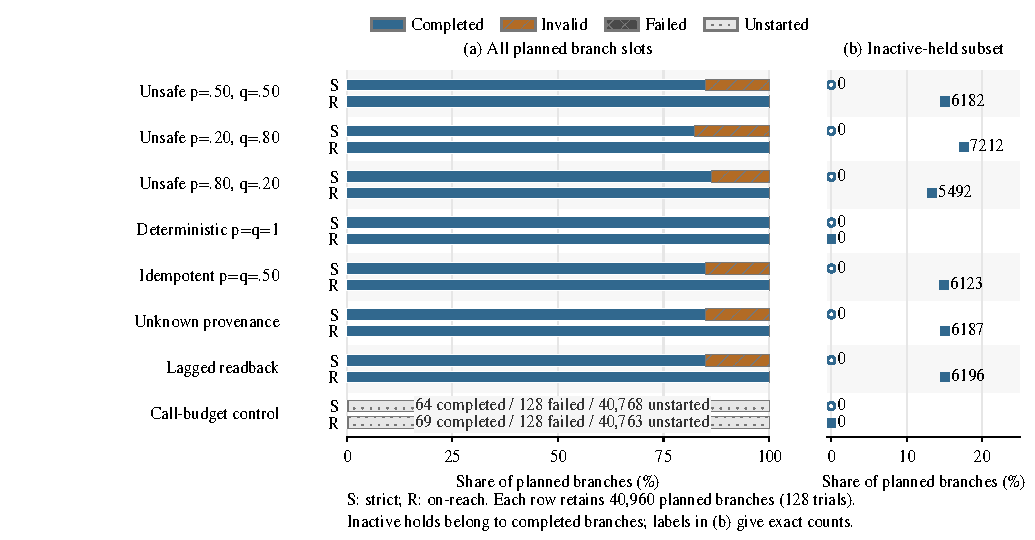
\includegraphics[width=\textwidth]{data-branch-disposition.pdf}
\caption{Disposition of all planned branches across eight mechanisms and two
games: 40,960 slots per row. Completed execution includes unknown target
evidence and known violations; it does not establish an available coefficient.
Failed and unstarted budget-control slots remain visible through exact counts.
Inactive holds are a subset of completed branches, shown separately.}
\label{fig:branches}
\end{figure*}

A standalone auditor importing no framework implementation checked the retained
trials, branches, 4,210 complete traces and all summary rows.
Its receipt binds the frozen source revision and original
52-file manifest. Derived tables retain every row separately from that sealed
collection; auditing made no generation calls.

Actual-call cost also depends on availability. The on-reach unsafe
$(0.5,0.5)$ stratum used 42,526 scripted calls for 128 available global-consequence
coefficient vectors, or 332.23 calls per vector, including factual capture and
independent endpoints. Each vector contains three jointly estimated players.
The lagged stratum spent 42,424 calls for zero such vectors; its cost-per-usable
vector ratio is undefined. Shared targets and interval variants do not multiply
the number of independent usable vectors. These are scripted-call costs, not
production latency or financial charges.

\begin{table*}[t]
\caption{All eight declared cases: on-reach retry coefficient for global
consequence, 128 planned repetitions per row. N/H denotes normal/Hoeffding.
Availability A and population-reference eligibility R each have denominator 128.
Flags denote correct directional detection for nonzero references and false
nonzero flags for zero references. Dashes denote undefined quantities;
0/0 denotes an undefined coverage rate. Hoeffding intervals are clipped to
$[-1,1]$, explaining the 0.773 mean width at $(0.8,0.2)$ versus the
unclipped 0.960 width at the two other stochastic unsafe settings.}
\label{tab:repeated}
\centering\footnotesize
\begin{tabular}{lrrrrr}
\toprule
Case $(p,q)$ or control & Reference & A ; R & Covered N / H & Mean width N / H & Flags N / H\\
\midrule
Unsafe $(0.5,0.5)$ & 0.375 & 128 ; 128 & 118/128 ; 128/128 & 0.226 / 0.960 & 128/128 ; 8/128\\
Unsafe $(0.2,0.8)$ & 0.120 & 128 ; 128 & 124/128 ; 128/128 & 0.154 / 0.960 & 123/128 ; 0/128\\
Unsafe $(0.8,0.2)$ & 0.720 & 128 ; 128 & 123/128 ; 128/128 & 0.218 / 0.773 & 128/128 ; 128/128\\
Deterministic $(1,1)$ & 0 & 128 ; 128 & 128/128 ; 128/128 & 0 / 0.960 & 0/128 ; 0/128\\
Idempotent $(0.5,0.5)$ & 0 & 128 ; 128 & 123/128 ; 128/128 & 0.244 / 0.960 & 5/128 ; 0/128\\
No provenance $(0.5,0.5)$ & 0.375 & 128 ; 128 & 120/128 ; 128/128 & 0.228 / 0.960 & 128/128 ; 7/128\\
Lagged readback $(0.5,0.5)$ & --- & 0 ; 0 & 0/0 ; 0/0 & --- & ---\\
Four-call cap $(0.5,0.5)$ & 0.375 & 0 ; 128 & 0/0 ; 0/0 & --- & ---\\
\bottomrule
\end{tabular}
\end{table*}

\begin{figure*}[t]
\centering
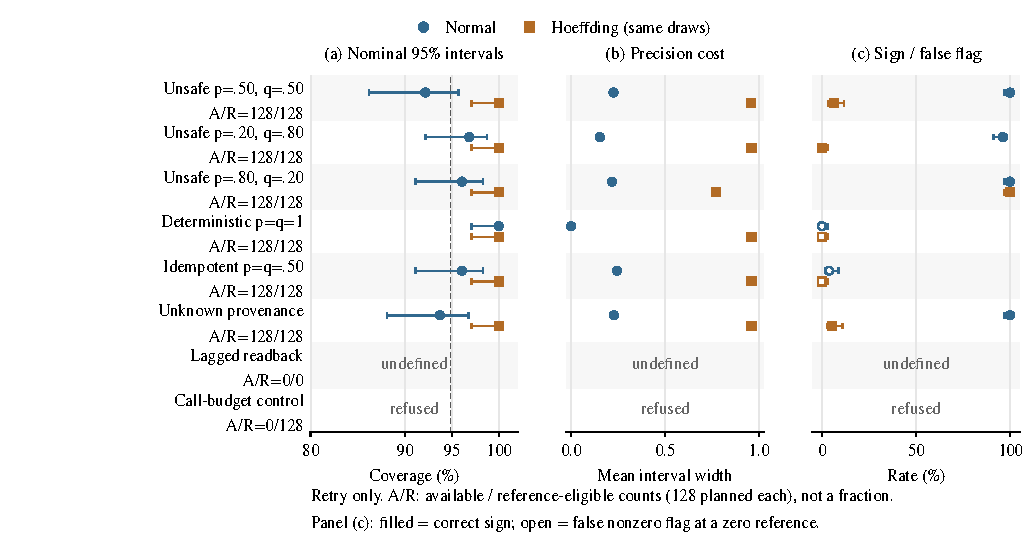
\includegraphics[width=\textwidth]{data-interval-tradeoffs.pdf}
\caption{On-reach global-consequence retry coefficient for all eight cases,
using identical draws for both interval methods. A/R denotes available and
population-reference-eligible counts, each from 128 planned trials. Coverage
and flag whiskers are 95\% Wilson uncertainty for repeated-trial rates, not
coefficient intervals. Filled flag markers indicate correct directional
detection; open markers indicate false nonzero flags for zero-reference
controls. Undefined evidence and budget refusals have no zero-valued markers.}
\label{fig:tradeoffs}
\end{figure*}

Table~\ref{tab:repeated} reports every declared mechanism for one specified
target and position, including unavailable controls.
Figure~\ref{fig:tradeoffs} places coverage beside interval width and detection
to expose their tradeoff without pooling targets or cases. At $(p,q)=(0.5,0.5)$,
the shared retry estimate had bias $-0.00269$ and RMSE 0.0611. Normal coverage
118/128 has a 95\% Wilson interval $[0.862,0.957]$; 128/128 has
$[0.971,1]$, not proof of perfect population coverage. The conservative
intervals sharply reduced weak-effect sign detection. For the consequence
stop dummy, normal false nonzero flags ranged from 0 to 14/128 across the six
assessable mechanisms; Hoeffding flags were 0/128 in each. The deterministic
zero-reference case yielded 128 normal point intervals; their correctness in
that case does not validate point intervals for stochastic outcomes.
With 128 repetitions, $[0.862,0.957]$ also shows why an observed 92.2\% rate
does not resolve a small departure from 95\% coverage. These runs are diagnostic
integration evidence, not a precise empirical ranking of near-nominal methods.
The finite-distribution calculation supplies a separate analytic check only
for its declared independent Bernoulli law.

Endpoint behavior was separately assessed. For the on-reach unsafe
$(0.2,0.8)$ global-consequence endpoint,
normal coverage was 92/128 (Wilson $[0.635,0.789]$), with 35 point intervals
and mean width 0.114. Exact-marginal differences covered 128/128, with mean
width 0.319. These finite results demonstrate the declared precision tradeoff;
they do not establish simultaneous coverage or calibration under live-model
dependence.

In the on-reach game, every lagged-consequence coefficient was refused as
unknown; every budget
coefficient was refused after unstarted slots, despite the latter's defined
ideal reference. Removing provenance preserved global-consequence availability
but refused all 128 linked-consequence coefficient vectors. All nondeterministic strict
coefficient vectors were unavailable and their population games undefined;
the fully deterministic strict control remained defined. One finite strict
interaction point at $(0.8,0.2)$ did not make that population interaction
defined. One strict linked-consequence endpoint without provenance was numeric
but reference-ineligible, giving coverage 0/0 rather than an accuracy result.
Pooled-coalition interaction diagnostics have no confidence interval
and supply no coverage or sign-detection result. The full summary retains
separate availability, reference eligibility, bias/RMSE, coverage uncertainty,
width, flags, endpoints, interactions and refusal rows for every target,
position, game and interval variant. Reused targets and variants are not
independent replications.

\subsection{Exploratory local-model validation}
A frozen installed Qwen3 4B checkpoint completed six validation cases,
two repetitions and two unchanged prompt profiles, using 59 actual calls
within a 72-call cap. No episode failed or remained unstarted. Model identity,
prompt/payload hashes, public traces and the exact source checkpoint are retained.
The original and revised profiles induced different action sequences; this
is not a pure reporting experiment or an attribution-method comparison.

\begin{table}[t]
\caption{Local-model validation with explicit claim denominators.}
\label{tab:model}
\centering\footnotesize
\begin{tabular}{lrr}
\toprule
Quantity & Original v1 & Revised v2\\
\midrule
Completed/planned episodes & 12/12 & 12/12\\
Actual calls/profile cap & 36/36 & 23/36\\
Definite final status claims & 12/12 & 0/12\\
Contradictions/assessable claims & 6/10 & 0/0\\
State satisfied/violated/unknown & 6/4/2 & 7/3/2\\
Linked satisfied/false/unknown & 6/4/2 & 5/5/2\\
\bottomrule
\end{tabular}
\end{table}

The revised profile's conditional contradiction rate is undefined, not zero
error. The original profile's 6/10 contradiction proportion has a descriptive
95\% Wilson interval of approximately $[0.313,0.832]$. Shared cases, fixed
profile order and two repetitions per case preclude interpreting this interval
as calibrated uncertainty over a broader population of tasks or models.
In the other-actor case, revised-profile readback satisfied state while
origin was external and action linkage false. In the expired-request case,
the original profile correctly described ineligibility but issued a refund;
its failure assessment contradicted achieved effect. Effect satisfaction and
eligibility-policy correctness are distinct targets.

A separate unblinded annotation pass within the AI-assisted development
workflow marked affirmative processing clauses in 10/12 original and 7/12
revised final rationales. Five of those
seven revised rationales also hedged independent verification. A statement
that a second attempt committed can be literally true while two effects
violate an exactly-one task. These annotations are descriptive; no independent
human verification or inter-rater reliability has been established. Unknown
structured fields do not ensure prose abstention. The saved auditor rejected
seven corrupted smoke copies without additional generation. Fixed profile order,
tiny sample size, shared fault conditions and an exposed validation family
limit interpretation. The held-out reserve was not generated.

\subsection{Matched three-model factual auditing}
A separate internally timestamped protocol froze source \texttt{bcd733d8},
model digests, unchanged profiles and wording before generation. Three small
local checkpoints (Qwen3 4B, Llama 3.2 3B and Gemma 3 1B), two profiles,
two new wording families,
seven exposed mechanisms and six repetitions gave 504 planned slots.
World/phase seeds were matched across model/profile cells; repetition blocks
randomized model, profile and case order. Temperature was 0.2, output cap 384
tokens, with thinking disabled and at most two tool attempts per episode.
CPU-only local Ollama used no paid API or real payment. These are fourteen
fixed case/wording cells, not 504 independent task samples. Family, size and
quantization are confounded; the earlier held-out reserve remains unused.
The frozen six-hour/1,512-call limits were not exhausted.

\begingroup\raggedright\footnotesize
Exact checkpoints: \nolinkurl{qwen3:4b-instruct-2507-q4_K_M};
\nolinkurl{llama3.2:3b-instruct-q4_K_M};
\nolinkurl{gemma3:1b-it-q4_K_M}.\par\endgroup

Five offline auditors score identical completed episodes, with no extra model
call: last public response; final structured assessment; readback without
provenance; an independently implemented contract/provenance reference; and
Consequa-X. The last two share information. Ledger gold uses a separate
discrete-time predicate; the reference uses an event sweep. This compares
factual information budgets without extra model calls; the separately frozen
trace-judge comparison follows below. This five-auditor analysis does not
measure causal attribution or a verify-before-retry controller.

All 504 slots started; 503 completed and one Llama v2 missing-provenance slot
failed strict-JSON parsing. That failure was retained without replacement.
There were 896/1,512 attempted calls, all with received responses, and no
transport failures, interruptions or unstarted slots. Collection finished
normally in approximately four hours 58 minutes. Definite coverage divides
claims by completed gold-assessable episodes; claim error divides wrong by
definite claims; correct yield divides correct by assessable episodes. Full
planned operational yield retains all 504 slots. Zero denominators remain
undefined and abstentions do not count as correct.

\begin{figure*}[t]
\centering
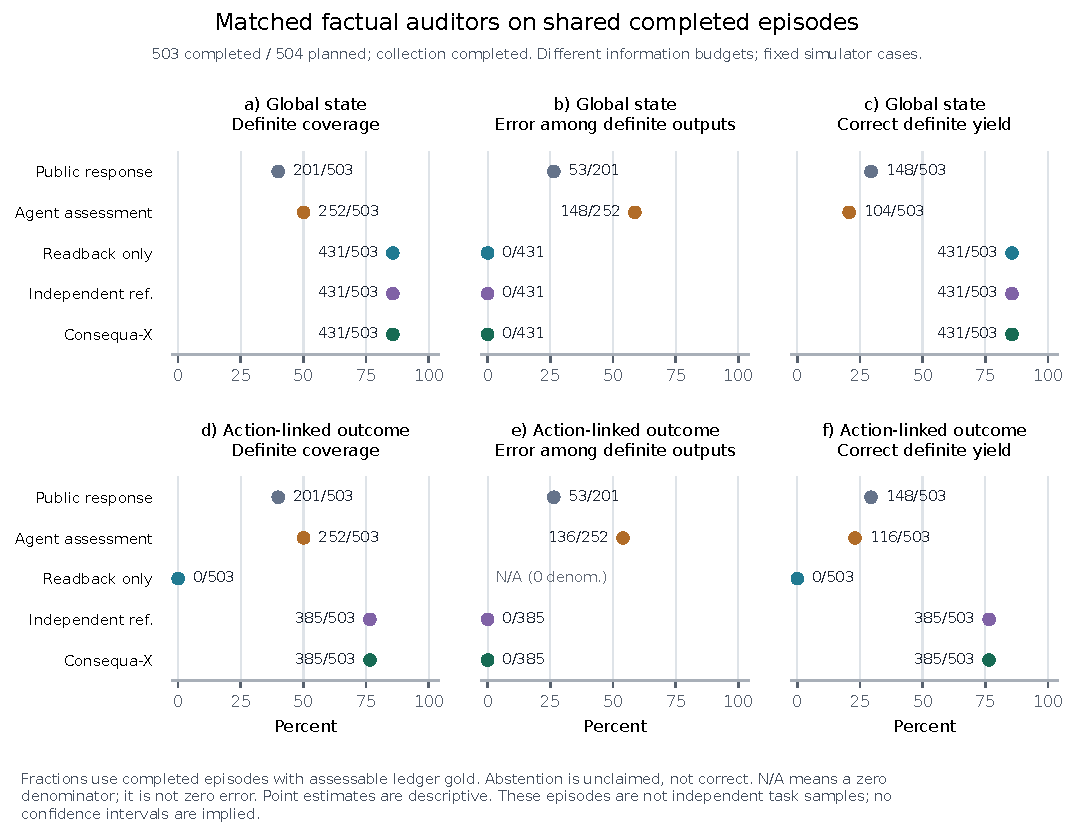
\includegraphics[width=\textwidth]{matched-baseline-metrics.pdf}
\caption{Matched factual auditors on shared completed episodes. Exact
fractions separate definite coverage, error among definite outputs and correct
yield for global state and action linkage. Auditors have declared different
information budgets; reference and Consequa-X share the same information.
Points are descriptive, without independent-task confidence intervals.}
\label{fig:matched-auditors}
\end{figure*}

Figure~\ref{fig:matched-auditors} retains every auditor. Response-only made
201 state claims, with 53/201 wrong and 148/503 correct yield; structured
self-report made 252, with 148/252 wrong and 104/503 yield. Readback, reference
and Consequa-X each made 431/503 correct state claims, with 0/431 observed
errors and 72 lag abstentions. For action linkage, response-only had 53/201
wrong, self-report 136/252, and readback-only abstained on all 503. Reference
and Consequa-X made 385/503 correct linked claims with 0/385 errors; the
remaining 118 comprise 72 lag and 46 omitted-provenance abstentions. Planned
state/linked yields for Consequa-X were 431/504 and 385/504.

Origin gold was assessable for 310/503 completed episodes, including five
excess-effect episodes that failed the exactly-one state contract. Reference
and Consequa-X made 216/310 correct definite origin claims (144 confirmed,
72 other-actor), with 0/216 wrong and planned yield 216/504. The 94 assessable
origin abstentions comprise 48 lag and 46 omitted-provenance cases; the other
193 completed episodes had unknown ledger-origin gold. Other auditors made no
origin claims. Complete reference/Consequa-X predictions, including abstention
and origin, agreed on 503/503 episodes. This parity supports implementation
correctness, without demonstrating advantage over an equally informed method.

\begin{figure*}[t]
\centering
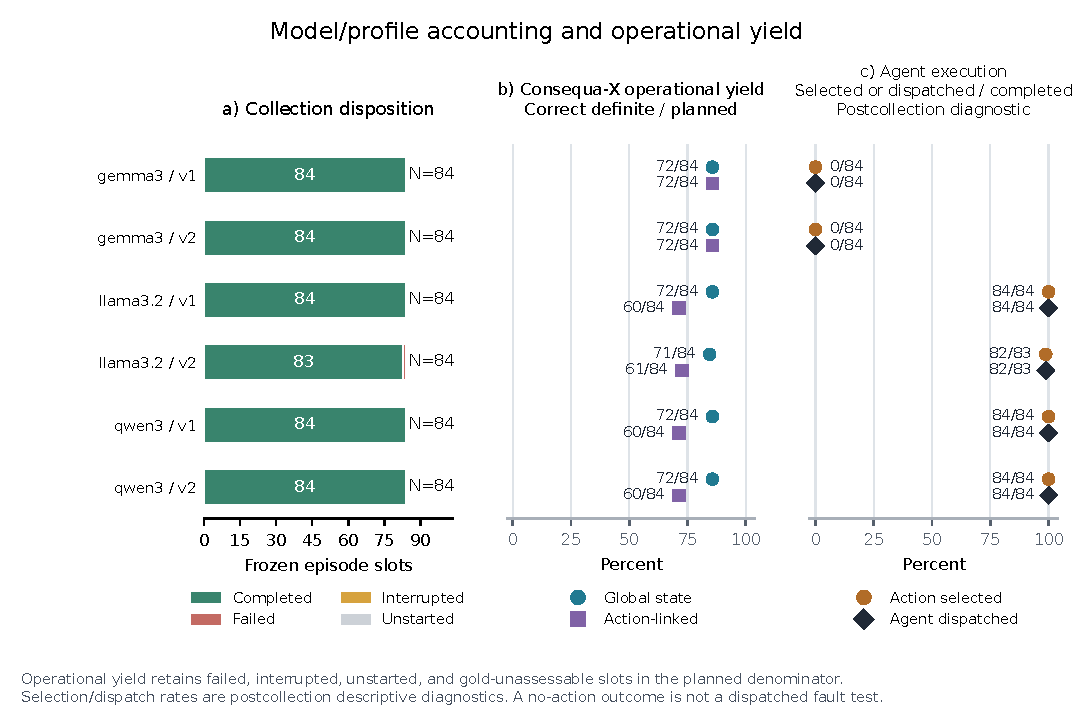
\includegraphics[width=\textwidth]{matched-model-disposition.pdf}
\caption{Model/profile accounting and execution. Operational yields retain
all 84 planned slots per group. The dispatch panel uses completed episodes and
is a post-freeze descriptive diagnostic. A no-action episode does not exercise
a dispatched fault. Full checkpoint tags and all fractions are retained with
the source figure inventory.}
\label{fig:matched-models}
\end{figure*}

Execution diagnostics were added descriptively after the first-six no-action
audit, without changing generation, primary metrics or stopping rules. Only
334/503 completed episodes dispatched an agent action (334/504 planned), with
392 tool attempts and 58 retries. Gemma dispatched 0/168 completed episodes;
Llama dispatched 166/167, with zero retries; Qwen dispatched 168/168, with
47 v1 and 11 v2 retries. An external actor can still create an effect during a
no-action episode. Empty-ledger correctness must not be described as refund
execution or fault handling. Figure~\ref{fig:matched-models} places these
execution rates beside semantic yield. Raw byte journals, every disposition,
source-bound inventories and condition/model/profile fractions are retained.
No pooled significance, population confidence interval, model ranking or
independent human annotation is established by this fixed simulator collection.

\subsection{Same-evidence local trace judge}
A separate protocol froze source \texttt{be842879}, aliased inputs, prompt,
checkpoint and budget before judge generation. It selected the 84 original
schedule slots with repetition zero after factual collection, retaining every
selected input; these span fourteen fixed wording/mechanism cells and
seventeen distinct public evidence patterns. The judge was the installed
Qwen3 4B checkpoint used in the factual study, at temperature 0.2, a 192-token
cap and thinking disabled. Each input received one call without repair or
replacement. The allowlisted input contained action/contract,
dispatch/response context and captured readback with scope, completeness,
watermark and provenance. Equality-preserving aliases hid identifiers;
generator/fault labels, reported assessments, rationales,
verification/explanation outputs and evaluator truth were excluded. The strict
output schema requested only state, action-linked satisfaction and origin.

All 84 selected traces completed in 84 local calls, with no failed,
interrupted, unavailable or unstarted slots. The judge made 60/84 definite
state claims: 9/60 were wrong, all false positives, giving 51/84 correct yield
and 24 abstentions. An automated public-reference rule qualified 43 state
claims as evidence-supported; eight other correct guesses lacked that
support. All 84 action-linked outputs were unknown: claim error is undefined,
not zero. Of 52 origin claims with assessable gold, 40 were correct and 12
wrong; eight additional definite origin outputs had unassessable gold and
receive no invented true/false label. Of the 40 correct origin claims, 24
were supported by the public rule and 16 were unsupported correct guesses.

\begin{figure*}[t]
\centering
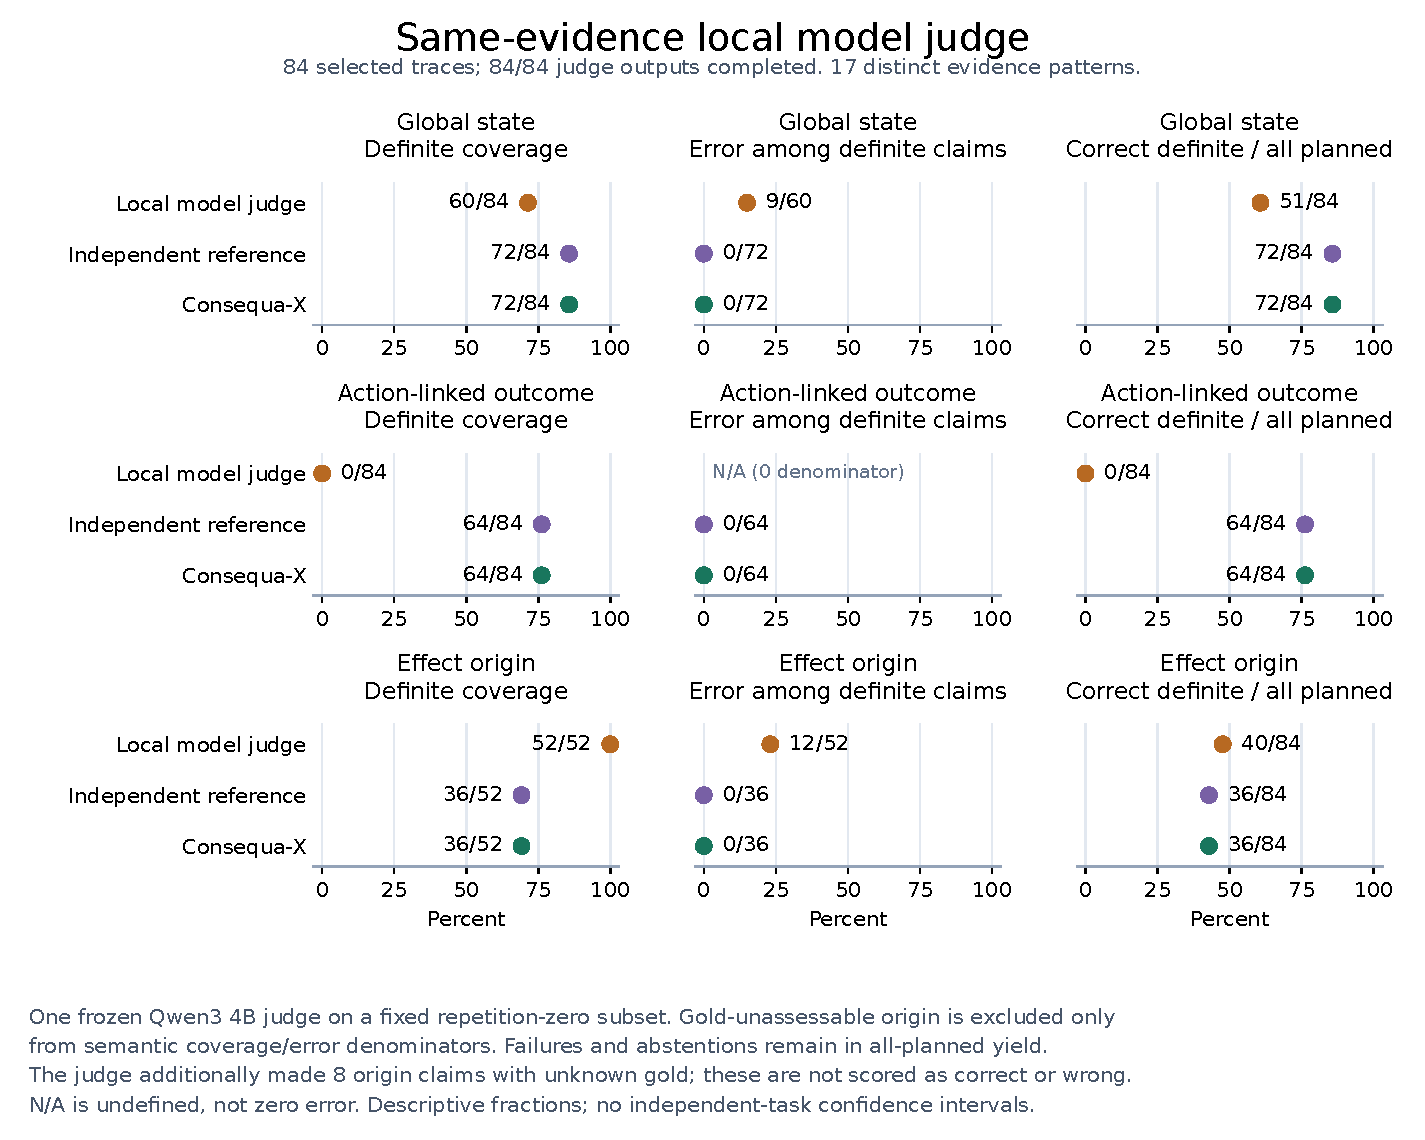
\includegraphics[width=\textwidth]{same-evidence-trace-judge.pdf}
\caption{Same-evidence local trace judging. Coverage uses gold-assessable
episodes, error uses definite claims with assessable gold, and correct
operational yield retains all 84 selected slots. Undefined zero-claim error remains undefined. Eight extra
origin claims with unassessable gold are retained separately. Points compare
one local judge and two equally informed deterministic implementations,
without independent-task intervals or a general model-superiority claim.}
\label{fig:trace-judge}
\end{figure*}

Reference and Consequa-X remained exactly equal, making 72/84 correct state,
64/84 correct action-linked and 36/52 correct assessable-origin claims, with
no observed wrong claims; selected-slot origin yield was 36/84. Hindsight
correctness therefore remains distinct from source-qualified explanation.
The subset is not held out or externally preregistered; repeated evidence,
one small judge sharing a generator family, and rule-based qualification
limit inference. This comparison supplies neither independent human
annotation nor population-level evidence about LLM judges
(Fig.~\ref{fig:trace-judge}).

\subsection{Maintained benchmark tool-state transfer}
A separately frozen, model-free experiment used the MIT-licensed maintained
tau3 corpus at \texttt{96a3ef92}: all 114 retail and 50 airline \texttt{base}
tasks in source order, with unchanged native tools, environments and
DB/environment evaluator~\cite{tau3tasks,tau3eval}. Three development tasks (retail 0; airline 19 and 20) exercised the adapter;
none were removed from the complete corpus. Four fixed controls replayed reference actions, omitted all writes,
omitted writes with a fabricated success acknowledgement, or altered the
first write's identity/scope while retaining later calls. All 656 cells
completed, with zero failures or unstarted cells and no model calls. Source/data, dependency bodies, protocols, starts and
result hashes were audited against the frozen source \texttt{7f6ef0c}.

Application contracts used each intended operation's payload and native
public preflight lookup. The read-only auditor received subsequent native
order, user or reservation lookups, without the complete reference action
list, gold DB or native reward. Contracts checked requested record fields,
not full financial settlement, policy or causal origin. The separate native
evaluator compared complete task DB end states after replaying the reference
on a fresh environment; it does not require a unique action sequence.
No dynamic user simulator, autonomous agent, communication criterion or NL
judge was evaluated.

\begin{figure*}[t]
\centering
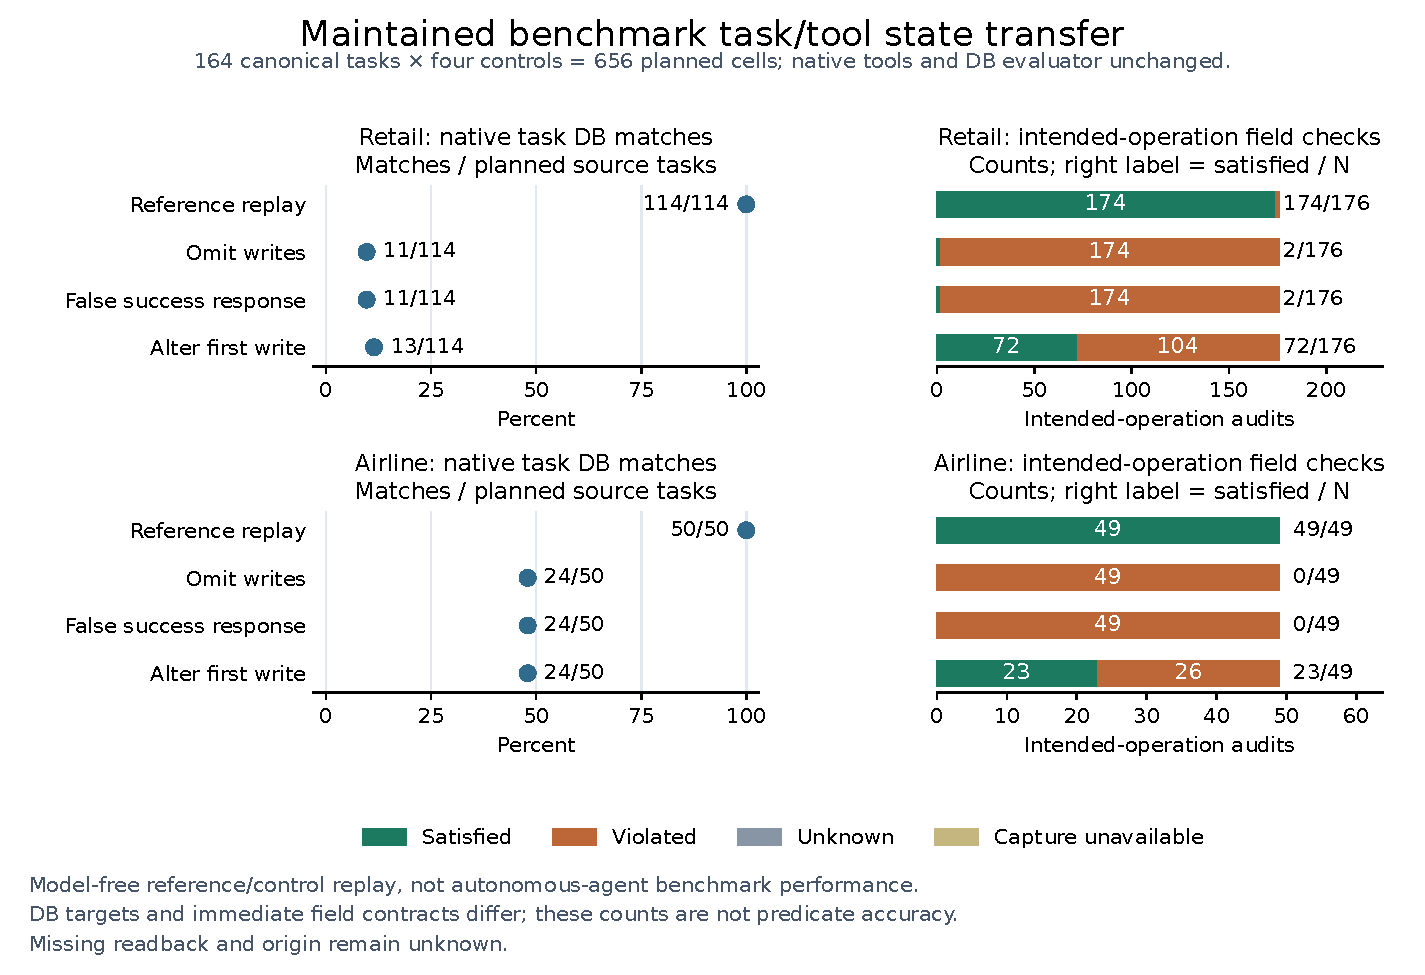
\includegraphics[width=\textwidth]{benchmark-state-transfer.pdf}
\caption{Model-free benchmark tool-state transfer. Task-level native DB
matching has denominators 114 retail and 50 airline tasks per control;
immediate requested-field checks have denominators 176 and 49 operations.
These targets and units differ. Reference DB equality is self-replay
consistency; field satisfaction is not independent predicate accuracy.
This figure reports no autonomous agent benchmark score or pass@k result.}
\label{fig:benchmark-transfer}
\end{figure*}

In reference/omit/fabricated-acknowledgement/alter-first-write order, native DB
matches were (114, 11, 11, 13)/114 for retail and (50, 24, 24, 24)/50 for
airline. Corresponding immediate field satisfactions were
(174, 2, 2, 72)/176 and (49, 0, 0, 23)/49. Ten retail and 24 airline reference
tasks contained no mutating call. All 900 operation captures were valid;
every withheld-readback check returned unknown, origin remained unknown
and assessment alignment unassessable. Native reference DB equality of
164/164 is not task correctness: retail task 64 has a rejected exchange
followed by a successful pending-order modification; task 105 has a
balance-rejected exchange and an unmeasured NL criterion requiring both
exchanges. These are retained without a dataset-bug claim. In tasks 22/110,
omitted writes can satisfy two individual address-field predicates because
the original address already matches a requested or restored state, without
proving mutation. The experiment supports cross-domain interface transfer,
with task-level and operation-level targets kept separate; it does not
establish production effectiveness or end-to-end benchmark performance
(Fig.~\ref{fig:benchmark-transfer}).

\subsection{Pinned native CAR comparison}
The earlier studies compare independent adaptations. A separate prospective
protocol at local source \texttt{940ebfc} executes native CAR 0.2.0,
revision \texttt{db90fa28}, without changing its contrastive, permutation,
NumPy percentile-bootstrap or SciPy normal-interval algorithms~\cite{carcode}.
The bridge supplies the same isolated refund world, planted factual
selection/retry/stop, continuation policy, outcome contract, captured
readback and on-reach game to both engines. Shared branch/phase seeds and
permutation order match draws rather than only nominal budgets. Native CAR
postdates the cited paper version; this is compatibility testing of the
pinned implementation through the declared bridge, not a reproduction of
the complete CAR paper or a live-model attribution benchmark.

Eight fixed mechanisms, two algorithms and 64 repetitions form 1,024 paired
groups, each containing two engine trials. Contrastive sampling uses 32
draws per factual position (96 slots per engine trial); Shapley uses 32
antithetic permutation pairs with one rollout per coalition and 16 extra
independent endpoints per arm (288 slots). There are 393,216 planned engine
draw slots. Independent finite Bernoulli enumeration supplies population
references. Repeats characterize fixed simulator settings: nominal 0.95
coverage has Monte Carlo standard error about 0.027 at 64 repeats, without
independent-task or multiplicity-adjusted inference.

Both engines share a cap on actual fresh policy calls, counting factual
capture and supplemental endpoints; held decisions consume no fresh calls.
The four-call control cannot increase its cap. Native rollout-budget charges,
deterministic prefix reconstruction, public tool re-execution and wall time
are separate cost fields. Native unknown labels and truncated vectors remain
raw diagnostics. An identical complete-method gate requires known factual
evidence and every planned draw before either primary coefficient vector is
released; it does not establish population-game validity from a finite sample.
Predeclared budget-start/refusal timing differences remain visible, while
other paired semantic mismatches stop collection without redraw.

\begin{figure*}[!t]
\centering
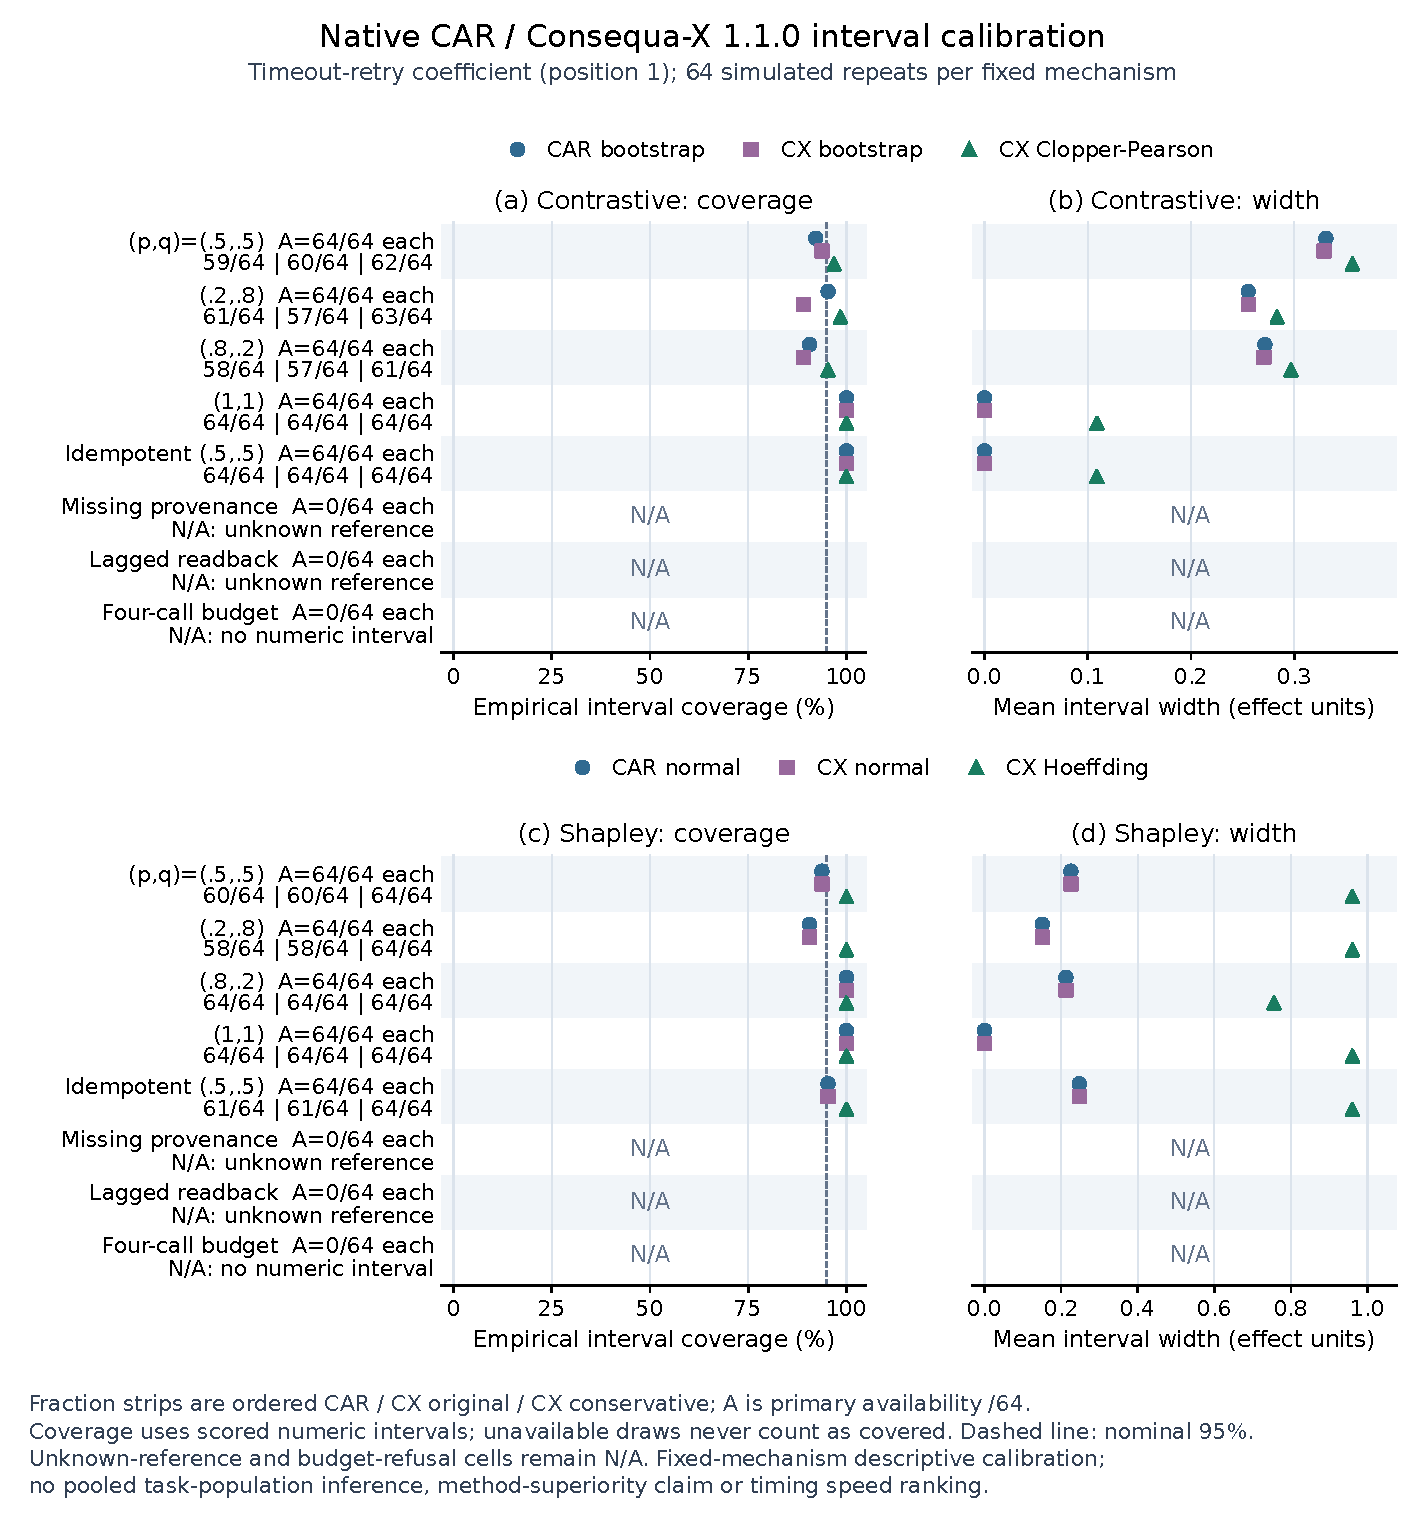
\includegraphics[width=\textwidth]{upstream-car-intervals.pdf}
\caption{Pinned native CAR and frozen Consequa-X 1.1.0 on the same timeout-retry
coefficient and replay draws. Every fraction uses 64 repetitions within a fixed
mechanism; A reports primary vector availability. Numerical coverage uses
reference-eligible available intervals, while missing evidence and budget
refusal remain undefined. Fraction order is CAR / Consequa-X original /
Consequa-X conservative. The budget control has coalesced native refusal
records, disclosed separately; none yields an eligible estimate. These are
conditional implementation/calibration checks, without a method ranking or
task-population claim.}
\label{fig:native-car}
\end{figure*}

Collection closed with all 1,024 paired groups and 2,048 engine files retained,
including all 393,216 canonical planned draw slots and zero redraws. The
independent audit checked every file, paired slot and source binding and
recomputed all summary rows without importing either implementation.
All factual traces and successful fresh-call totals match in all 1,024 pairs.
Both engines release 640 paired coefficient vectors and withhold 384;
every eligible paired point estimate agrees exactly. All non-budget draws
agree semantically. Unknown-provenance, lag and budget groups remain visible
with zero primary availability.

At the $p=q=0.5$ timeout-retry coordinate, native bootstrap coverage is
59/64 with mean width 0.331, compared with 60/64 and 0.329 for the independent
bootstrap adaptation. Its Clopper--Pearson alternative covers 62/64 at width
0.356. Native and adapted normal Shapley intervals both cover 60/64 at width
0.225; Hoeffding covers 64/64 at width 0.960. Finite bootstrap resampling
implementations remain distinct. Figure~\ref{fig:native-car} displays all
eight mechanisms at that coordinate; all three coordinates and 144 summary
rows remain in the artifact. These descriptive repeats do not establish a
method ranking or precise population calibration.

The audit found one collector deviation: in 64 native contrastive budget
groups, concurrent zero-spend refusals coalesce under one failed canonical
slot. Their 6,144 canonical slots are 40 known, 64 failed and 6,040 unstarted.
These labels do not identify actual coroutine starts one-to-one: source and
retained refusal records support 2,048 first-coalition invocations, with
40 completed and 2,008 refused. Individual refused-coroutine identities were
not retained. All 64 affected vectors are already ineligible; no accepted
estimate or successful-call cap changes. This limits refused-attempt
attribution, without changing the frozen records or silently amending the plan.

Each engine uses 209,666 successful fresh scripted policy calls, including
factual capture and endpoints, with zero live model calls. The native bridge
records 845,672 deterministic reconstruction/probe worlds and 968,304 tool
dispatches. These counters are adapter work, separately recorded rather than
independently reconstructed from full bridge histories. CX completed replay
worlds and preflights have different scopes. Wall times include worker
contention and bridge overhead, so they do not establish intrinsic speed.

\subsection{Offline conformance across the breaking 2.0 release}
The preceding experiments remain frozen on 1.1.0/schema 0.1. To assess a
narrow migration boundary, source \texttt{f64bf49} and a separate protocol
were committed before processing all 503 retained factual traces. The
original 504-slot schedule and its failed strict-JSON policy output remain
unchanged; no replacement trace was generated. This is an exposed-data,
post-hoc conformance study, with zero new model calls or action executions.
Isolated 1.1.0 and 2.0.0 environments load the exact pinned implementations.
Each legacy observation is bound by its recorded ID, source and watermark;
fresh verification uses that same stored observation rather than a new
readback. Each version's action-linked target helper is used, without
substituting a nonempty target-ID list for its provenance-qualified result.

All 503 traces migrate, round-trip through schema 1.0 and preserve the
declared legacy structural projection. Migration preserves recorded
conclusions by construction; separately, fresh 2.0 verification agrees with
fresh frozen-1.1.0 verification on all legacy receipt fields, state, origin,
action-linked target and assessment alignment. The recorded old analysis
and explanation also agree with their frozen recomputation. Every primary
comparison is 503/503 with zero processing failures or unavailable
comparisons. This is 503 usable inputs per 504 historical slots, not a
disagreement assigned to the missing input. Agreement includes unknown:
fresh state is satisfied on 257, violated on 174 and unknown on 72.
Alignment is consistent on 48, contradicted on 108 and unassessable on 347.

Diagnosis codes are deliberately not a canonical invariant. They agree on
228/503 traces and change on 275: 2.0 adds
\texttt{UNASSESSABLE\_ASSESSMENT} in all 275 and removes
\texttt{CONSISTENT\_OUTCOME} in 24 of those. Migrated and freshly verified
explanations show the same changes. Target-match metadata is nonempty on
144 receipts, empty on 287 and unavailable on 72; these categories are
neither action-linked accuracy nor independent labels for the new fields.
All 503 migrate to \texttt{relative\_ms}, because schema 0.1 did not record a
clock origin. The receipt-reproduction gate checks status, origin, effect
IDs and attributable IDs; it does not certify every added metadata field.

An independent artifact auditor checks hashes, all slot identities,
structural projections and refund evidence arithmetic without importing the
framework or collection runner. Its JSON-level checks are distinct from the
runner's recorded framework round-trip assertion. This single-action refund
corpus supplies no conformance claim for general multiple-action traces,
custom verifiers, polling, controllers or the changed replay transport.
Canonical agreement is a migration result, not new predicate accuracy or
end-to-end equivalence of the two releases.

\section{Discussion and Limitations}
The evidence protocol supports different, inspectable claims about responses,
state, origin and intervention effects. Its refusal rules withhold affected
numerical outputs when captured factual evidence or a planned draw is invalid
or unavailable, but can sharply reduce availability. Availability can depend
on interventions and must remain visible beside numerical results. Conservative
intervals do not make undefined games numeric, resolve missing evidence, or
remove the need to assess the actual sampling law.

The refund experiments remain a narrow scripted simulator, and no real payment
API was evaluated. The local trace judge adds a same-evidence model comparator;
the native retail/airline replays add maintained benchmark tool-state transfer,
not autonomous benchmark performance or a second production-domain study.
Declared source authority and watermarks are not authenticated transactional
guarantees. The three small generator checkpoints and one overlapping judge
cover exposed development/validation mechanisms. Fresh wording, seventeen
judge evidence patterns and canonical task/control replays do not establish
held-out fault transfer or independent task-population inference. State and
linked targets sharing outcomes are not independent replications. Claims
about hidden reasoning cannot be inferred from reported assessments.

Three evaluation gaps remain. First, extend the completed factual ablations,
local trace-judge comparison, model-free tool-state transfer and pinned
native CAR bridge to a live verify-before-retry controller, full autonomous
benchmark runs and joint causal/structural attribution. The bridge tests
native estimators on a matched scripted game; it does not reproduce CAR's
full live-agent evaluation. Further comparisons require matched information,
targets and call budgets; state satisfaction, source-supported origin and
causal intervention effects need distinct reference labels. Report duplicate
effects, false success, availability, attribution accuracy and actual cost.
Joint context/fault attribution must expose infrastructure variables to every
applicable method. The current trace judge is one small local checkpoint,
not an independently validated population of stronger judges.

Second, assess bounded polling on an eventually consistent readback: poll
until its declared watermark covers the horizon or a predeclared wait budget
expires, then retain unknown. Report availability against wait time, read
count and latency. Polling cannot promise finality or exactly-once execution
under arbitrary late commits. The retained lag control uses one insufficient
readback and yields zero consequence estimates; a polling result has not been
measured. A safe real-service study would use provider test mode, isolated
accounts and injected acknowledgement faults; counterfactual replay would
remain in an isolated simulator or a separately validated digital twin.

Third, sample independently authored held-out task and fault-composition
families, with an explicit task-population precision analysis and independent
blinded double annotation. The 504-slot study supplies conditional repeated
observations, not 504 independent task samples. More seeds cannot replace
domain diversity. At least 1,000 independent repetitions per selected
simulator setting would better resolve interval coverage, with simultaneous
uncertainty and modern bounded-mean comparators. No polling effectiveness,
full live-agent causal-method comparison or human annotation agreement is
claimed here. Offline 2.0 conformance reuses exposed saved evidence; its
503 agreements do not add independent task samples or validate new features.

The retained cost record counts actual scripted calls and refusals; the repeated
study used 628,535 calls and zero model calls. It does not measure per-call
verification latency, trace-size overhead, real-API charges or cost per usable
production estimate. Those measurements belong in the next evaluation.

\section{Conclusion and Artifact Availability}
Consequa-X provides a reusable evidence core and auditable replay adapters for
separating reported assessments, external outcomes, origin and intervention
effects. The retained studies expose uncertainty failure, precision costs,
variable-length restrictions and prose/structured-status disagreement. Matched
factual auditing additionally measures the limits of response/status proxies
and agreement with a same-information reference, including abstentions.
The same-evidence local judge exposes unsupported correct guesses, while
maintained benchmark replays separate task DB equality from immediate operation
fields. Neither supplies a general method ranking or independent human labels.
Pinned native CAR runs additionally show exact point agreement for 640
eligible paired vectors, with unavailable groups and a refusal-recording
deviation disclosed. Offline 2.0 migration preserves canonical conclusions
on 503 retained traces while changing diagnosis codes on 275; the earlier
experiments retain their evaluated version and source pins.
The useful result is a reproducible protocol/software artifact with measured
limits, without claiming a new estimator or general method superiority.

Version 2.1.1, now branded ConseqaX, is publicly available under MIT on PyPI~\cite{artifact},
with source and retained research records in the public repository at
\url{https://github.com/Devrajsinh-Jhala/consequa-x}. Its release record binds
the distribution hashes to build source \texttt{b73ecd0}. The earlier breaking
2.0 release introduced schema 1.0, multiple actions and assessments, declared
time bases and immutable keyword-only records. Target matches and findings
move into verifier receipts; explanation selects the latest assessment per
action. Migration has the separate offline conformance check above. Capture,
polling and retry-advice interfaces are later product capabilities, not
interventions measured by the frozen 1.1.0 experiments. The 2.1 line adds
verifier composition, OpenTelemetry interchange and optional framework
integrations. Models, the built-in refund verifier, explanation, target helper
and numerical estimator modules remain unchanged from the measured 2.0
source, but the public verification wrappers now accept multiple readbacks.
The 2.0 result therefore does not validate all 2.1.1 execution paths.
Release-specific installed-artifact checks cover Windows Python 3.11--3.15
and one emulated Alpine Linux/Python 3.14 guest; macOS remains untested.
The release retains one live engineering smoke run per integration:
OpenAI Agents SDK and LangChain use local Ollama, while Claude Agent SDK
uses authenticated remote Haiku with an in-process SDK MCP tool server.
These runs test wiring, not comparative task accuracy, deployed MCP services
or OpenTelemetry collectors. They are separate from the frozen scientific
experiments. A DOI-backed immutable research archive
has not been established.

The earlier experiments retain source pins \texttt{9e2dcbb} (original
calibration), \texttt{0d8ec0b} (shared draws), \texttt{2c4adfe}
(enumeration/local validation) and \texttt{0bd744d} (repeated sampling).
The three-model factual study used \texttt{bcd733d8}; the judge protocol
declared \texttt{be842879}; tool-state transfer froze \texttt{7f6ef0c},
with maintained external source \texttt{96a3ef92}; native CAR used
\texttt{940ebfc} with upstream \texttt{db90fa28}. Full revisions, protocol
hashes and inventories remain study-specific. Those experiments used
the 1.1.0 runtime and schema 0.1~\cite{experimentartifact}. The 2.0 estimator
modules retain their numerical implementations, but record models, verifiers,
explanation and replay transport have changed. The offline migration study
uses separate source \texttt{f64bf49} and a separately committed protocol;
byte identity of estimator modules alone does not establish end-to-end
equivalence. Later releases do
not rerun, reseal or relabel the frozen studies. Readback trust and completeness remain application
responsibilities. GitHub Actions remains disabled.
Framework imports and offline examples require no model credentials or required
runtime dependencies. All reported payments are simulated; model weights are
identified rather than redistributed.

\section*{AI Assistance and Verification Disclosure}
Generative AI assistance was used for software development, research-source
inspection, rationale annotation and manuscript drafting. Recorded automated
checks cover retained-evidence accounting, analytic references, numerical
implementations and document compilation. They do not constitute independent
human replication or blinded annotation. The rationale labels remain unblinded
and exploratory. The author is responsible for the paper's claims and any
venue-required disclosure; no independent human validation is asserted.

\appendices
\section{Declared-Game Properties and Test Evidence}
\label{app:games}
\textbf{Strict-game partiality.} In the declared three-position mechanism,
let $N=\{s,r,t\}$ be selection, timeout retry and final stop. If $p<1$, the
coalition $\{r\}$ requests a retry that is unreachable with probability
$1-p>0$ when fresh selection declines. If $q<1$, coalition
$\{s,t\}$ holds selection and requests a final stop that is unreachable with
probability $1-q>0$ when the fresh timeout decision stops. With compatible
decisions, normal execution, adequate budget and known outcomes, the full strict
coalition game is structurally defined if and only if $p=q=1$ in this mechanism.
In particular the full strict game is partial at every interior $(p,q)$ and
ordinary full-game Shapley is undefined there. Conditioning on valid replay
would define a different game. A finite sample with no invalid draw cannot
establish zero population invalid probability.

\textbf{On-reach allocation.} Fix finite factual positions, an intervention
mapping and a continuation law. Suppose each coalition terminates almost surely,
all reached held decisions are compatible, and a bounded measurable numeric
outcome exists almost surely. Ignoring holds beyond normal termination then
defines $v(S)=\mathbb{E}[X_S]$ for every coalition. Its ordinary Shapley values
obey efficiency, symmetry, the null-player property and linearity. To see
efficiency, sum the marginal contributions along each permutation: they
telescope to $v(N)-v(\varnothing)$, and averaging preserves the equality.
Relabelling permutations gives symmetry; zero marginals give the null-player
property; linearity follows from linearity of each difference and of averaging.
These properties belong to this declared game. They establish neither causal
identifiability nor nonnegative normalized responsibility. Unknown observations,
incompatible holds and provider failures remain outside these assumptions.
Finite independently sampled coalition values can give a nonzero estimate for
a true null player, and an independently sampled endpoint need not equal the
sum of finite estimated shares.
Uniform forward permutations and their reverses each have a uniform marginal.
With unbiased coalition samples, their paired average is unbiased for the
declared Shapley value. Independent pairs, rather than individual walk steps,
are the sampling units for the bounded-mean interval.

\textbf{Test mapping.} C1 is exercised by external-actor and absent-provenance
tests in \texttt{test\_verification.py} and conflicting-observation tests in
\texttt{test\_graph\_identity.py}. C2 is exercised by
\texttt{test\_refund\_interactions.py}, the exact-rational analytic checker,
and retained enumeration controls. C3 is exercised by unknown-draw and
exhausted-budget tests in \texttt{test\_decision\_shapley.py}, plus the
saved-evidence branch audit. Tests establish behavior in their stated cases,
not correctness of an untrusted source or a real-service policy.

\section{Supporting Audit Inventory}
Raw assertion counts are retained for reproducibility rather than treated as
evidence strength: 3,283,523 for the shared-draw audit, 27,277 for the enumeration
audit, 44,698,925 for repeated sampling, and 2,227 for the local validation.
These counts depend on data volume and auditor implementation. More informative
checks include independently recomputed summaries, exact-rational analytic
references, source-bound inventories, refusal denominators and rejected
semantic corruptions. None supplies independent human verification.

\balance
\begin{thebibliography}{99}
\bibitem{car} J. Shah, ``Causal Agent Replay: Counterfactual Attribution for
LLM-Agent Failures,'' arXiv:2606.08275, v1, Jun. 2026.
\bibitem{pccc} R. Meng, ``Policy-Conditioned Counterfactual Credit for Verifiable
Reinforcement Learning of Long-Horizon Language Agents,'' arXiv:2606.05263, v1,
Jun. 2026.
\bibitem{causalloss} A. Sharma, ``CausalLoss-Fin: Attributing Financial-Agent
Loss to Decisions and Infrastructure Faults,'' arXiv:2609.25960, v1, Sep. 2026.
\bibitem{verified} I. K. Mansoor, A. Phadke, and P. Rana, ``Verified Tool Calls
Improve LLM Agent Reliability Under Non-Atomic Failures,'' arXiv:2608.02645,
v1, Jul. 2026.
\bibitem{operability} Z. Wang, ``Callability Is Not Operability: Controlled
Interface Interventions for LLM Agents,'' arXiv:2608.23628, v2, Aug. 2026.
\bibitem{whoandwhen}
S. Zhang \emph{et al.}, ``Which Agent Causes Task Failures and When? On Automated Failure Attribution of LLM Multi-Agent Systems,'' in \emph{Proc. 42nd Int. Conf. Machine Learning}, PMLR, vol. 267, 2025, pp. 76583--76599. [Online]. Available: \url{https://proceedings.mlr.press/v267/zhang25cq.html}
\bibitem{prov}
L. Moreau and P. Missier, Eds., ``PROV-DM: The PROV Data Model,'' W3C Recommendation, Apr. 30, 2013. [Online]. Available: \url{https://www.w3.org/TR/2013/REC-prov-dm-20130430/}
\bibitem{agenttool}
A. Trofimov and B. Novikov, ``When Tool Calls Succeed but Workflows Fail: Anomalies at the Agent-Tool Boundary,'' arXiv:2609.15397v1, 2026. [Online]. Available: \url{https://arxiv.org/html/2609.15397v1}
\bibitem{limbo}
J. Li, ``Where Does Exactly-Once Live? Model, Harness, and Tool-Contract Effects on Duplicate Side Effects in LLM Agents,'' arXiv:2609.29095v1, 2026. [Online]. Available: \url{https://arxiv.org/html/2609.29095v1}
\bibitem{helland}
P. Helland, ``Idempotence Is Not a Medical Condition,'' \emph{Communications of the ACM}, vol. 55, no. 5, pp. 56--65, 2012, doi: 10.1145/2160718.2160734.
\bibitem{vogels}
W. Vogels, ``Eventually Consistent,'' \emph{Communications of the ACM}, vol. 52, no. 1, pp. 40--44, 2009, doi: 10.1145/1435417.1435432.
\bibitem{appworld}
H. Trivedi \emph{et al.}, ``AppWorld: A Controllable World of Apps and People for Benchmarking Interactive Coding Agents,'' in \emph{Proc. 62nd Annu. Meeting Association for Computational Linguistics}, vol. 1, 2024, pp. 16022--16076, doi: 10.18653/v1/2024.acl-long.850.
\bibitem{toolsandbox}
J. Lu \emph{et al.}, ``ToolSandbox: A Stateful, Conversational, Interactive Evaluation Benchmark for LLM Tool Use Capabilities,'' in \emph{Findings of the Association for Computational Linguistics: NAACL 2025}, 2025, pp. 1160--1183, doi: 10.18653/v1/2025.findings-naacl.65.
\bibitem{taubench}
S. Yao, N. Shinn, P. Razavi, and K. Narasimhan, ``$\tau$-bench: A Benchmark for Tool-Agent-User Interaction in Real-World Domains,'' arXiv:2406.12045v1, 2024. [Online]. Available: \url{https://arxiv.org/html/2406.12045v1}
\bibitem{brown}
L. D. Brown, T. T. Cai, and A. DasGupta, ``Interval Estimation for a Binomial Proportion,'' \emph{Statistical Science}, vol. 16, no. 2, pp. 101--133, 2001, doi: 10.1214/ss/1009213286.
\bibitem{betting}
I. Waudby-Smith and A. Ramdas, ``Estimating Means of Bounded Random Variables by Betting,'' \emph{Journal of the Royal Statistical Society Series B: Statistical Methodology}, vol. 86, no. 1, pp. 1--27, 2024, doi: 10.1093/jrsssb/qkad009.
\bibitem{shapley} L. S. Shapley, ``A Value for N-Person Games,'' RAND
Corporation, P-295, 1952, doi: 10.7249/P0295.
\bibitem{clopperpearson}
C. J. Clopper and E. S. Pearson, ``The Use of Confidence or Fiducial Limits Illustrated in the Case of the Binomial,'' \emph{Biometrika}, vol. 26, no. 4, pp. 404--413, 1934, doi: 10.1093/biomet/26.4.404.
\bibitem{hoeffding} W. Hoeffding, ``Probability Inequalities for Sums of
Bounded Random Variables,'' Journal of the American Statistical Association,
vol. 58, no. 301, pp. 13--30, 1963.
\bibitem{tau3tasks}
Sierra Research, ``tau2-bench: Maintained retail and airline task corpus,''
MIT software, commit 96a3ef92329baf908ffe9dfe188cea34e8701d2a, 2026.
[Online]. Available:
\url{https://github.com/sierra-research/tau2-bench/tree/96a3ef92329baf908ffe9dfe188cea34e8701d2a}
\bibitem{tau3eval}
Sierra Research, ``Native environment evaluator,'' tau2-bench, same pinned
commit, 2026. [Online]. Available:
\url{https://github.com/sierra-research/tau2-bench/blob/96a3ef92329baf908ffe9dfe188cea34e8701d2a/src/tau2/evaluator/evaluator_env.py}
\bibitem{carcode}
J. Shah, ``Causal Agent Replay,'' software ver. 0.2.0, commit
db90fa28b97164c35e7c524e4597b8cbdb3035af, 2026. [Online]. Available:
\url{https://github.com/jaineet17/causal-agent-replay/tree/db90fa28b97164c35e7c524e4597b8cbdb3035af}
\bibitem{experimentartifact} D. Jhala, ``Consequa-X,'' MIT Python distribution,
ver. 1.1.0, Oct. 17, 2026. [Online]. Available:
\url{https://pypi.org/project/consequa-x/1.1.0/}
\bibitem{artifact} D. Jhala, ``ConseqaX,'' MIT Python distribution,
ver. 2.1.1, Oct. 19, 2026. [Online]. Available:
\url{https://pypi.org/project/consequa-x/2.1.1/}
\end{thebibliography}
\end{document}
